\documentclass{report}
\usepackage[utf8]{inputenc}
\usepackage[a4paper, total={7in, 10in}]{geometry}
\usepackage{graphicx}
\usepackage[parfill]{parskip}
\usepackage{amsmath}
\usepackage{wrapfig}
\usepackage{subfig}
\usepackage{titlesec}

\titleformat{\chapter}[display]
{\normalfont\huge\bfseries}{\chaptertitlename\ \thechapter}{20pt}{\Huge}
\titlespacing*{\chapter}{0pt}{0pt}{40pt}


\graphicspath{ {./Images/} }
\setlength{\parindent}{0em}

\title{Computer Vision} 
\author{Xin Wang}

\begin{document}
\par
\maketitle
\medskip

\tableofcontents

%%%%%%%%%%%%%%%%%%%%%%%%%%%%%%%%%%%%%%%%%%%%%%%%%%%%%%%%%%%%%%%%%%%%%%%%%%%%%%%%%%%%%%%%%%%%
\chapter{Image Formation}

A digital image is formed from three components:
\begin{enumerate}
    \item Lighting 
    \item Reflectance 
    \item Optics and Sensors
\end{enumerate} 

\section{Lighting}

Lighting has several properties of concern:
\begin{itemize}
    \item Location 
    \item Intensity of light 
    \item Spectrum of light
\end{itemize} 

There are many different sources of light. Four commonly used models to describe
light sources are:
\begin{itemize}
    \item \textbf{Point Light Source}: The light is inside the scene at a
    specific location only and it shines light equally in all directions. An example
    is be a table lamp.
    \item \textbf{Area Light Source}: The light source comes from a rectangular
    area and projects light from one side of the rectangle. An example is a
    florescent light fixture in a ceiling panel. 
    \item \textbf{Sun Light Source}: The light is outside the scene and far
    enough away that all rays of light are basically from the same direction. 
    An example is the sun in an outdoor scene.
    \item \textbf{Spotlight Light Source}: The light is focused and forms a
    cone-shaped envelop as it projects out from the light source. An example is
    a spotlight in a theatre. 
\end{itemize}

\section{Reflectance}

\begin{wrapfigure}[10]{r}{0.45\linewidth}
\centering
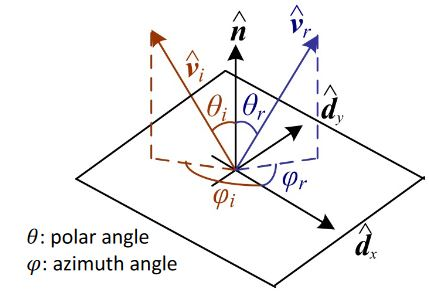
\includegraphics[width=6cm]{BRDF.JPG}
\caption{BRDF model}
\label{fig:myfig}
\end{wrapfigure}

A general model for modelling reflectance is the
\textbf{Bidirectional Reflectance Distribution Function (BRDF)}. The model
describes how much light arriving at incident direction is emitted in
reflected direction. 
$$
f_r\left(\theta_i, \sigma_i, \theta_r, \sigma_r, \lambda\right) = \frac{dL_r}{dE_i}
$$
where:
\begin{itemize}
    \item $\theta_i$ and $\sigma_i$: Incident direction
    \item $\theta_r$ and $\sigma_r$: Reflected direction
    \item $\lambda$: Wavelength
    \item $dL_r$: Output power 
    \item $dE_i$: Input power 
\end{itemize}

\pagebreak

Considering the two ideal cases of reflection: \textbf{Diffuse reflection} and
\textbf{Specular reflection}
\begin{itemize}
    \item \textbf{Diffuse reflection}: 
    \begin{figure}[h!]
        \centering
        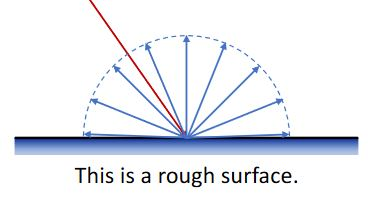
\includegraphics[width=.2\linewidth]{Diffuse reflection angle.JPG}
        \qquad
        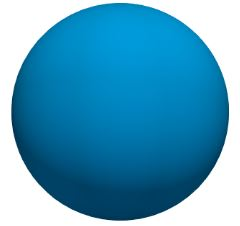
\includegraphics[width=.1\linewidth]{Diffuse reflection view.JPG}
    \end{figure}

    The light is scattered uniformly in all directions so the BRDF is constant:
    $$
        f_r\left(\theta_i, \sigma_i, \theta_r, \sigma_r, \lambda\right) = f_r(\lambda)
    $$

    This effect on the viewed image is similar to the appearance of a rough
    surface.
    
    \item \textbf{Specular reflection}: 
    \begin{figure}[h!]
        \centering
        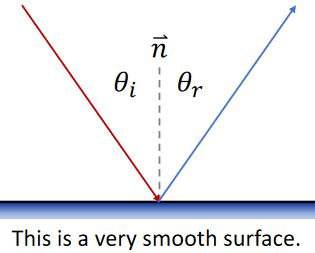
\includegraphics[width=.15\linewidth]{Specular reflection angle.JPG}
        \qquad
        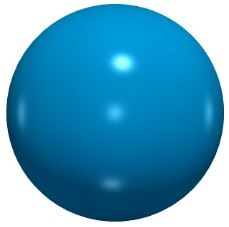
\includegraphics[width=.1\linewidth]{Specular reflection view.JPG}
    \end{figure}

    The light is reflected in a mirror-like fashion. The reflection and incident directions are symmetric with respect to the
    surface normal $\vec{n}$: $\theta_r = \theta_i$
\end{itemize}

For the majority of cases in the real world, there is a combination of
\textbf{diffuse reflection}, \textbf{specular reflection} and \textbf{ambient
illumination}. Ambient illumination accounts for general illumination which may be
complicated to model such as the inter-reflection between walls in a room and
distant light sources as seen in sunny outdoor environments.

This observation is formally state in the \textbf{Phong Reflection Model} which
is an empirical model in computer graphics that describes how a surface reflects
light as a combination of ambient, diffuse and specular components. 
\begin{figure}[h]
    \centering
    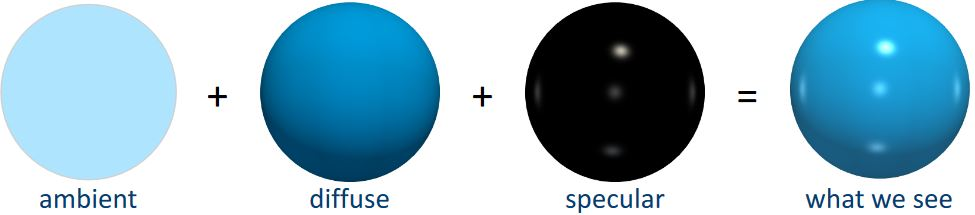
\includegraphics[width=10cm]{Phong reflection model.JPG}
\end{figure}

\subsection{Computer graphics}

There is an unique relationship between computer graphics and computer vision
similar to the relationship of writing and reading. Computer graphics is
concerned with generating images while computer vision is concerned with
intepreting images. 

This relationship is particularly valuable as computer graphics in
photorealistic games can be used to generate data i.e. images + labels for
training computer vision algorithms. 

\section{Optics}

Camera sensors imitates the human eye which are human sensors. In the human eye,
there are two types of neural cells in the retina: 
\begin{itemize}
    \item \textbf{Cone cells}: Colour vision and functions in the bright light. 
    \item \textbf{Rod cells}: More sensitive to the light but monochromatic and
    functions in the dim light like night time. 
\end{itemize}

Camera sensors are very much the same: \textbf{Charge-coupled Device (CCD)} and
\textbf{Complementary Metal-oxide Semiconductor (CMOS)}.

\subsection{Colour Filter Arrays (CFA)}

A color filter array (CFA) or color filter mosaic (CFM) is a mosaic of tiny
color filters placed over the pixel sensors of an image sensor to capture color
information.  

The most common CFA is the most single-chip digital image sensors used in
digital cameras to create a colour image is the \textit{Bayer Filter Mosaic}.
The Bayer Filter Mosaic is arraged to mimic the human eyes i.e. most sensitive
to green light with $50\%$ green, $25\%$ red and $25\%$ blue.

The RGB of different cameras may be different, i.e. with different sensitivities
to wavelengths. This different colour sensitivity is why the same picture with
different cameras would look different.

\subsection{Bayer Colour Filter}

With its arrangement, only one colour is available at each pixel. The other two
colours can be interpolated from neighbouring pixels. Through this
interpolation at each pixel, the RGB values can be obtained. 
\begin{figure}[h]
    \centering
    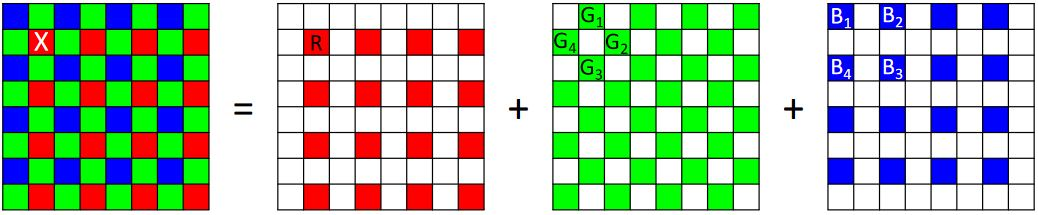
\includegraphics[width=10cm]{Bayer colour filter.JPG}
    \caption{Bayer colour filter and interpolation}
\end{figure}

\subsection{Demosaicing}

A demosaicing algorithm is a digital image process used to reconstruct a full
colour image from incomplete colour samples output from an image sensor overlaid
with a CFA.

A simple method is bilinear interpolation where the red value of a non-red pixel
is computed as the average of the two or four adjacent red pixels, and similarly
for blue and green.  
\begin{figure}[h]
    \centering
    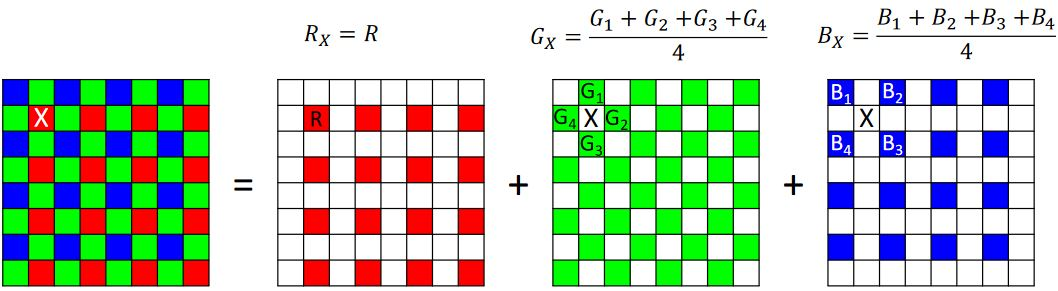
\includegraphics[width=10cm]{Demosaicing algorithm.JPG}
\end{figure}

\subsection{Colour spaces}

\begin{wrapfigure}[10]{r}{0.35\linewidth}
    \centering
    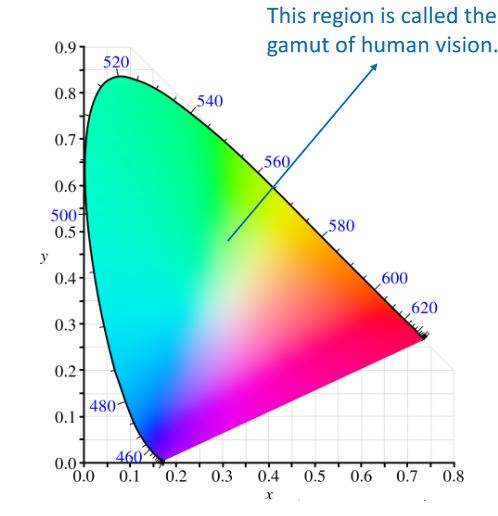
\includegraphics[width=5cm]{Colour space repre.JPG}
    \caption{CIE 1931}
\end{wrapfigure}

Colour spaces are mathematical models describing the way colours can be
represented. Colour spaces can be seen as a box containing all possible colours that can be
produced by mixing primary colours of RGB. 

The CIE 1931 XYZ was created by the International Commission on Illumination and
represents the colour space using the primary colours X, Y and Z. 
\begin{align*}
    x &= \frac{X}{X+Y+Z} \\
    y &= \frac{Y}{X+Y+Z} \\
    z &= \frac{Z}{X+Y+Z}
\end{align*}

There are various different forms colour spaces such as sRGB, HSV and CMYK.  All
these colour spaces can represent the same colour, but using different
primary colours or coordinate systems.

\subsection{Quantisation}

Quantisation is the process that maps continuous signal to discrete signal. For
colours, color quantization reduces the number of colors used in an image. This
is important for displaying images on devices that support a limited number of
colors and for efficiently compressing certain kinds of images.

It is important to note that numerical errors occur during quantisation,
which depends on the number of bits used. The more bits, the less quantisation
error.

%%%%%%%%%%%%%%%%%%%%%%%%%%%%%%%%%%%%%%%%%%%%%%%%%%%%%%%%%%%%%%%%%%%%%%%%%%%%%%%%%%%%%%%%%%%%
\chapter{Image Filtering}

The goal of using filters is to modify or enhance image properties and/or to
extract valuable information from the pictures such as edges, corners, and
blobs.

There are various types of image filters such as:
\begin{itemize}
    \item Identity filter
    \item Low-pass/Smoothing filters: Moving average filter or Gaussian filter 
    \item High-pass/Sharpening filters 
    \item Denoising filter: Median filter
\end{itemize}

\section{Smoothing Filters: Moving Average Filter}

A moving average filter moves a window across the signal and calculates the
average value within the window. A \textbf{filter kernal} is specified to
indicate what values are averaged in the moving average filter. A filter
kernal \footnote{https://en.wikipedia.org/wiki/Kernel\_(image\_processing)}
is a small matrix used for blurring, sharpening, edge detection etc. 

In images, the moving average filter removes high frequency signal e.g. noise or
sharpness. This operation results in a smooth but blurry image. For example,
consider a \textbf{box blur} kernal and its effect:

\begin{minipage}{7in}
    \centering
    \raisebox{-0.5\height}{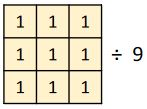
\includegraphics[height=0.5in]{Box blur.JPG}}
    \hspace*{.2in}
    \raisebox{-0.5\height}{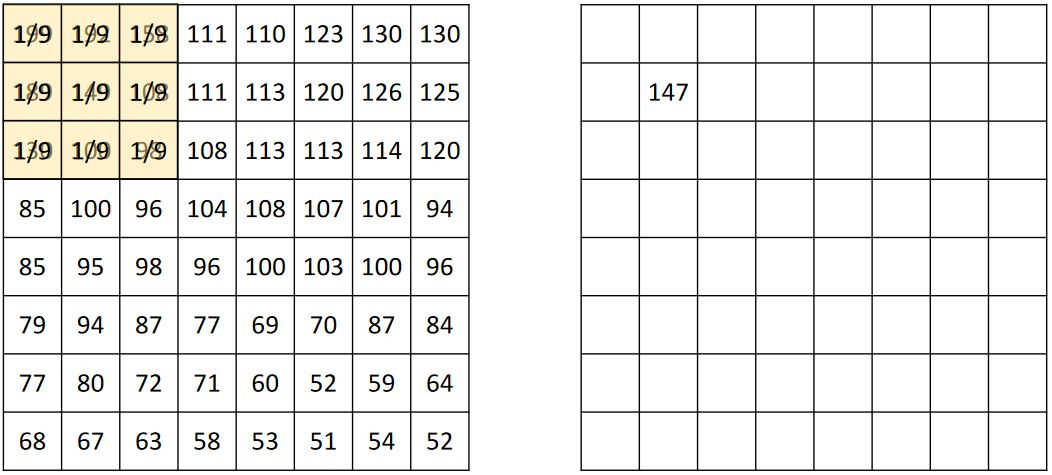
\includegraphics[height=1.5in]{Box blur calculation.JPG}}
\end{minipage}

Due to the nature of this method of calculations, the output image will be
smaller than the input image. The boundary pixels are generally dealt with using
padding of various methods such as constant value, mirroring values etc. The
following example uses 0 padding for its boundary pixels. 

\begin{minipage}{7in}
    \centering
    \raisebox{-0.5\height}{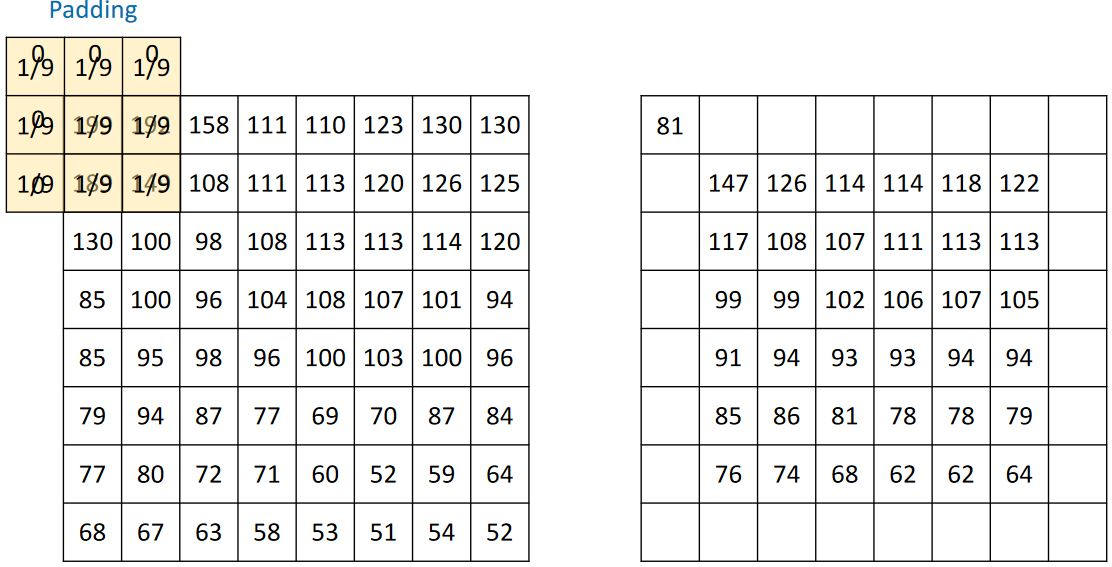
\includegraphics[height=1.5in]{Zero padding.JPG}}
    \hspace*{.2in}
    \raisebox{-0.5\height}{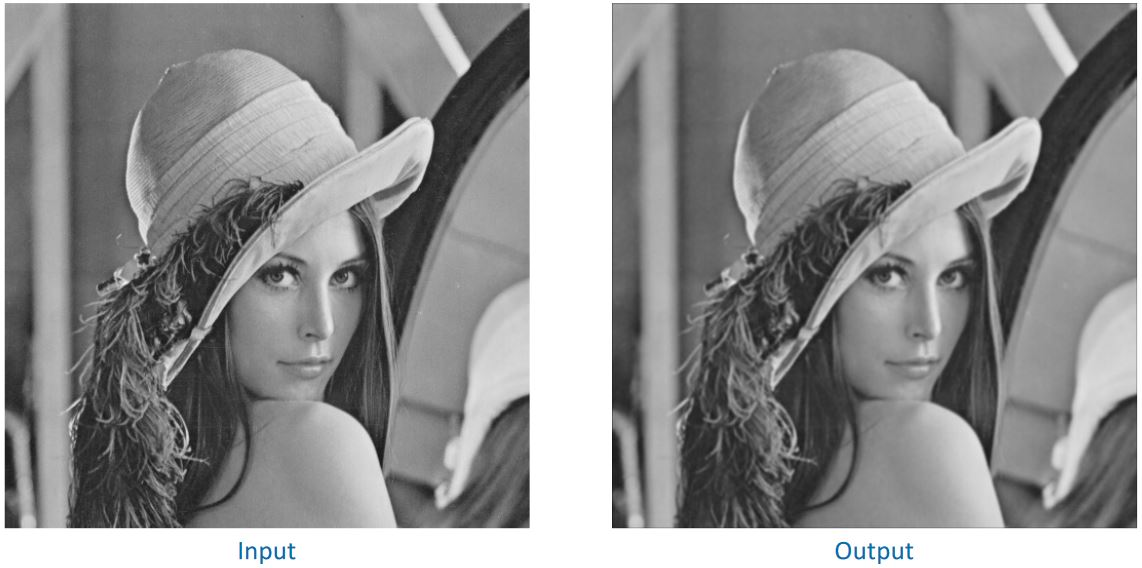
\includegraphics[height=1.5in]{Blur images.JPG}}
\end{minipage}

By increasing the size of the kernal e.g. into a $7 \times 7$ matrix, the image
will become blurrier. 

\vfill

\subsection{Brute Computational Complexity}

Note that: \textit{Image size}: $N \times N$ where $N$ is the number of pixels and
\textit{Kernal size}: $K \times K$ where $K$ is size of the filter kernal matrix 
\begin{itemize}
    \item There are $N^2$ pixels 
    \item At each pixel, there are $K^2$ multiplications and $K^2 - 1$ summations.
    \item In total, there are: $N^2 K^2$ multiplications and $N^2(K^2 - 1)$
    summations 
    \item Complexity is: $O(N^2 K^2)$
\end{itemize}

\subsection{Separable filter}

If a big filter can be separated as the consecutive operation of two small
filters, then the first filter can be applied to the the input image then the
second filter. For example, consider the previous blur filter kernal divided
into two smaller filters:
\begin{figure}[h]
    \centering
    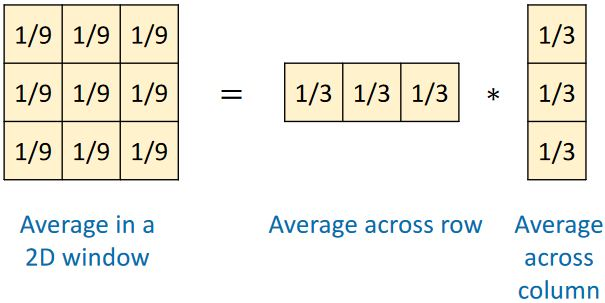
\includegraphics[width=6cm]{Blur separable filter.JPG}
\end{figure}

This calculation procedure results in the same result as the previous result:

\begin{minipage}{7in}
    \centering
    \raisebox{-0.5\height}{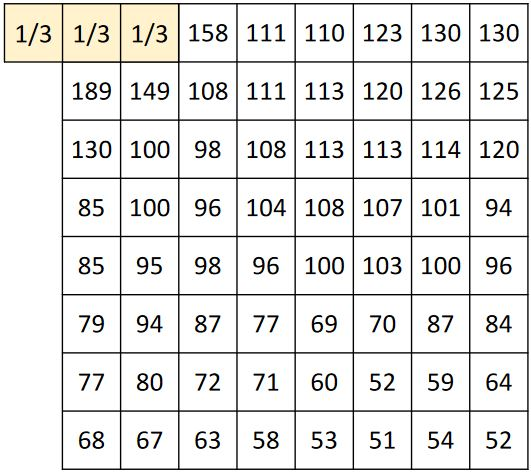
\includegraphics[height=1.5in]{X separable filter 1.JPG}}
    \hspace*{.2in}
    \raisebox{-0.5\height}{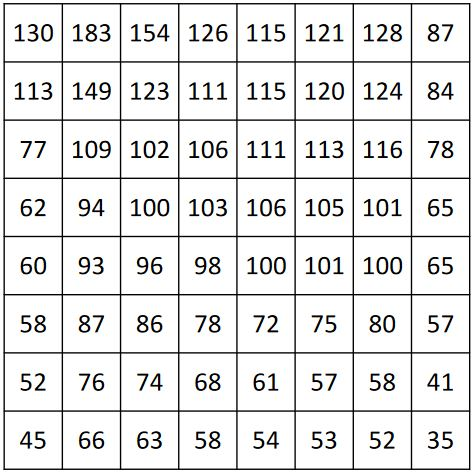
\includegraphics[height=1.5in]{X separable filter 2.JPG}}
\end{minipage}

\begin{minipage}{7in}
    \centering
    \raisebox{-0.5\height}{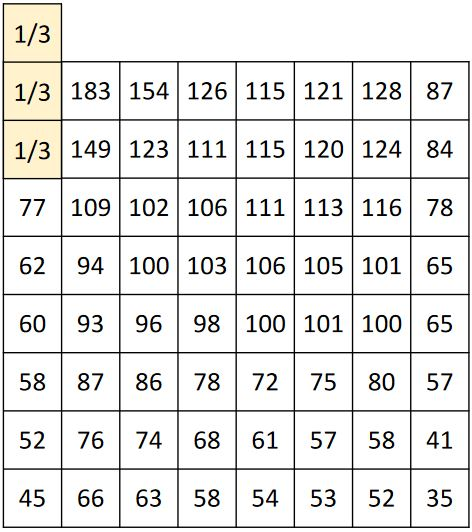
\includegraphics[height=1.5in]{Y separable filter 1.JPG}}
    \hspace*{.2in}
    \raisebox{-0.5\height}{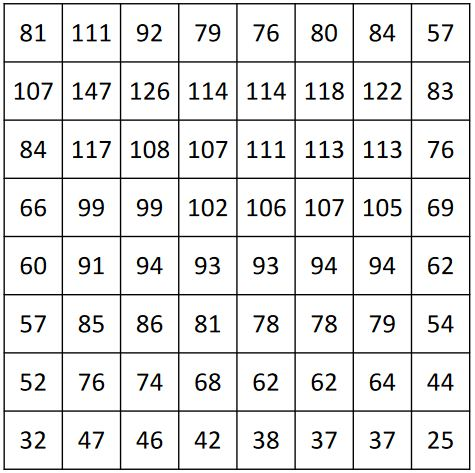
\includegraphics[height=1.5in]{Y separable filter 2.JPG}}
\end{minipage}

\subsection{Separable filter complexity}

Note that: \textit{Image size}: $N \times N$ where $N$ is the number of pixels
and there are two filter kernals: $1 \times K$ and $K \times 1$.
\begin{itemize}
    \item There are $N^2$ pixels 
    \item At each pixel, there are $K$ multiplications and $K - 1$ summations.
    \item In total, there are: $2N^2 K$ multiplications and $2N^2(K - 1)$
    summations 
    \item Complexity is: $O(N^2 K)$ which is faster than the previous $O(N^2 K^2)$
\end{itemize}

\section{Identity Filter}

The \textbf{Identity Filter Kernal} simply returns the same value of the image
i.e. the input and output image is the same.

\section{Smoothing Filters: Gaussian Filter}

The Gaussian Filter uses a 2D Gaussian Distribution as its filter kernal:
$$
    h(i,j) = \frac{1}{2\pi \sigma^2} e^{- \frac{i^2 + j^2}{2\sigma^2}}
$$

The 2D Gaussian filter is a separable filter, equivalent to two 1D Gaussian
filters with the same $\sigma$, one along x-axis and the other along y-axis:
\begin{align*}
    h(i,j) &= h_x(i) * h_y(j) \\
    h_x(i) &= \frac{1}{\sqrt{2\pi}\sigma}e^{-\frac{i^2}{2\sigma^2}}
\end{align*}

\section{High-pass Filters}

There are various methods of designing high-pass filters including using
low-pass filters as seen in Design 1.
\begin{figure}[h]
    \centering
    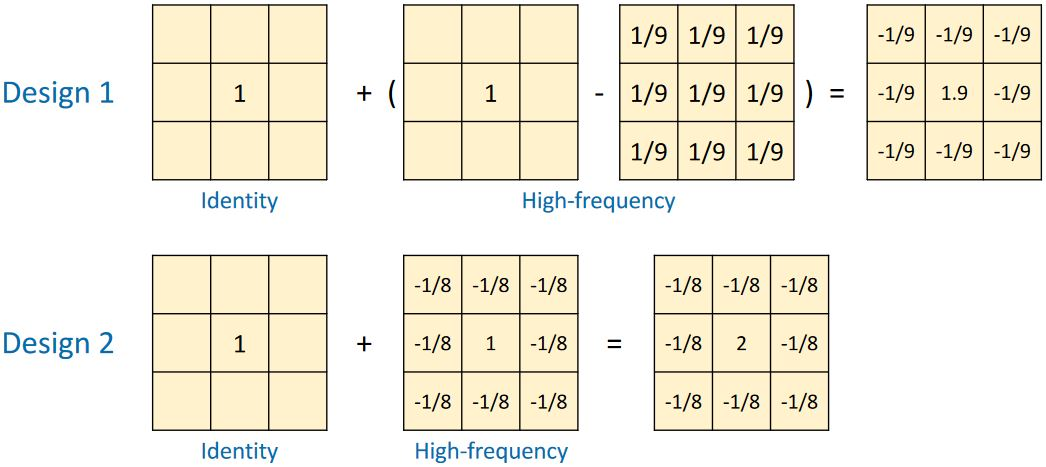
\includegraphics[width=10cm]{High pass.JPG}
\end{figure}

\section{Denoising Filters: Median Filter}

Median filters are non-linear filters that is often used for denoising an image.
A common method of performing median filter is to move the sliding window and
replacing the centre pixel using the \textit{median value} in the window.
\begin{figure}[h]
    \centering
    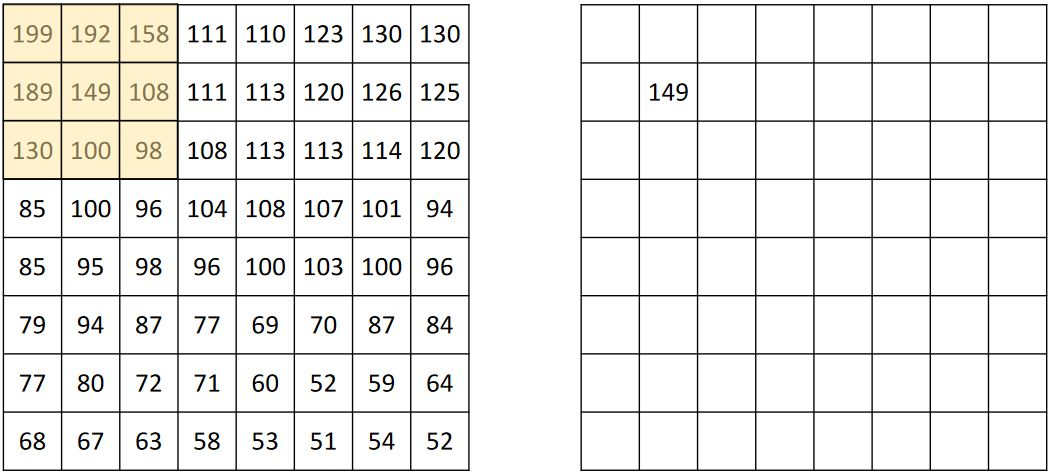
\includegraphics[width=10cm]{Median filter.JPG}
\end{figure}

\end{document}